\question{}

จงพิจารณานิยามของลำดับ (ordering) ในการท่องต้นไม้ค้นหาแบบทวิภาค (Binary search tree) 
ที่แตกต่างกันดังต่อไปนี้

\marginnote{%
    \textbf{ตัวอย่าง} เช่นจากรูปต้นไม้ตัวอย่างนี้

    \begin{center}
        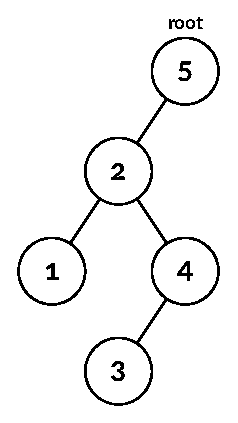
\includegraphics[width=0.6667\linewidth]{figures/quickfire_central_regional_bfsdfs.eps}
    \end{center}

    \begin{itemize}
        \item จะมี Pre-order traversal ordering เป็น $[\mathrm{5, 2, 1, 4, 3}]$
        \item และจะมี Breadth-first search ordering ได้สองรูปแบบ 
            ได้แก่ $[\mathrm{5, 2, 1, 4, 3}]$ และ $[\mathrm{5, 2, 4, 1, 3}]$
    \end{itemize}
}

\begin{itemize}
    \item \textbf{Pre-order traversal}
    ของโครงสร้างข้อมูลต้นไม้ค้นหาทวิภาค (Binary search tree) คือการใช้อัลกอริทึม 
    Depth-first search (DFS) เพื่อประมวลผลโหนดแต่ละโหนดของต้นไม้หนึ่งตามลำดับดังต่อไปนี้ 
    (โดยนับเริ่มต้นจากราก (root) ของต้นไม้)

    \begin{enumerate}
    \item compute โหนดตัวเอง
    \item recursively compute โหนดในกลุ่ม Subtree ทางซ้ายของโหนดตัวเอง
    \item recursively compute โหนดในกลุ่ม Subtree ทางขวาของโหนดตัวเอง
    \end{enumerate}

    \item \textbf{Breadth-first search ordering} 
    ของโครงสร้างข้อมูลต้นไม้ทวิภาค (Binary tree) คือลำดับการท่องต้นไม้ตามอัลกอริทึม 
    Breadth-first search (BFS) (\textbf{หมายเหตุ:} โดยมีเงื่อนไขกำหนดให้เริ่มต้นจากรากของต้นไม้) 
\end{itemize}

\noindent
\textbf{\uline{โจทย์}} สมมติว่ามีต้นไม้ค้นหาแบบทวิภาค (Binary search tree) $T$ อยู่ต้นหนึ่ง
ซึ่งพบว่ามีลำดับ Pre-order traversal เป็น $[\mathrm{7, 2, 1, 4, 3, 6, 5, 9, 8, 10, 11}]$\;
อยากทราบว่าต้นไม้ $T$ นี้จะมี Breadth-first search (BFS) ordering 
ที่เริ่มต้นจากรากได้ต่างกันทั้งหมด\uline{กี่รูปแบบ}?
